The Central Committee and the State Council promulgated the reform of the RMB exchange rate formation mechanism on July 21, 2005, the RMB exchange rate was no longer pegged to a single dollar, and fluctuated according to the market supply and demand. After August 11, 2015, the correlation between the RMB and the dollar index has declined. In 2016, the annual depreciation of RMB is about 6.67%, against a basket of currency depreciation rate is 5.13%. But the degree of marketization of the RMB in 2016 significantly increased, and gradually drops out of the "dollar anchor." RMB exchange rate change, as China's international financial relations and even the normal development of economic relations, is an important link and plays an increasingly important role. Therefore, it has a vital significance to correct analysis and forecast the exchange rate and its volatility for the economic subject of financial policy and investment and financing decision-making undoubtedly. Also, to predict the RMB exchange rate better, it is very important to choose a satisfactory model.
Many domestic scholars have studied this based on time series measurement method. Which model of ARIMA model, ARCH model or GARCH model is more appropriate for the exchange rate fluctuations has been controversial. The paper of Zhang Zhongjie (2005) suggested that the exchange rate change was fit into ARIMA (2,4,5) model. Hui Xiaofeng (2005) argued that there was a GARCH effect in the time series of RMB / USD, and the GARCH (1,1) model was suitable for RMB / USD modeling, Xu Shaoqiang and Li Yaming(2007) used the ARMA model to forecast the exchange rate of the euro and yen of a basket of currencies. Then calculated the future exchange rate of the yuan against the US dollar according to the RMB benchmark exchange rate formula, and the forecast results were carried out. Liu Shuling (2008) selected data of the changes in the daily parity of RMB against the US dollar from July 25, 2005 to November 1, 2007. It is estimated that the GARCH (1,1) model and the ARMA (1,1) model are all suitable. Cui Aimei(2009) showed that the RMB exchange rate volatility had certain leverage effect and the RMB exchange rate did not have the characteristics of floating exchange rate regime through the TGARCH model empirical study. Luo Xun (2009) analyzed the exchange rate volatility model established form the data after the reform of China's exchange rate system. The study shows that there existed ARCH effect in China's foreign exchange market and GARCH (1) was susitable.
It is not difficult to find that the data of previous studies are mostly old, while the appropriation of the model will change with the background of the times and the change of the data. In recent years, the international situation has been changed largely, so we select the latest data ,daily data from July 2005 to June 2017 of RMB exchange rate, to empirically research on the ARCH model, ARIMA model and GARCH model and to compare which forecasting model of RMB is more suitable for China and the development situation of this time.
\documentclass[12pt, a4paper, titlepage]{article}
\usepackage{amsthm}
\usepackage{amsmath}
\usepackage{amsfonts}
\usepackage{amssymb}
\setlength{\textwidth}{6.25in}
\usepackage{graphicx}
\usepackage{xcolor}
\usepackage{listings}
\lstset{numbers=none,
numberstyle=\tiny,
keywordstyle=\color{blue!70}, 
commentstyle=\color{red!50!green!50!blue!50},
frame=shadowbox,
rulesepcolor=\color{red!20!green!20!blue!20},
basicstyle=\ttfamily\small,
escapeinside=`', %将中文放在`和'之间,可以在lstlisting环境中准确的显示中文
}
\title{Financial Data Analysis Group Project\\
}
\author{Yufei Li  \\
	32014150004  \\
	\and 
	Yinan Wu \\
	32014150003 \\
	\and
	Ke Zhang\\
	32014150002\\
	\and
	Tianyunzi Chen\\
	32014020199
	}

\date{} 

\begin{document}
\maketitle

\begin{abstract}

\end{abstract}

\tableofcontents 

\section{Introduction}


\section{Data Source and Data Description}
\subsection{Data Source}

\subsection{Data Description}
We first use monthly USD/CNY exchange rate data from 1981-01-01 to 2017-06-01 to plot a trend figure shown as figure \ref{monthly}. According with the news, China used to set fixed exchange rate mechanism before 2015-07-21, the volatility of exchange rate was small. After that date, China started exchange rate regime reforming: announced a move away from the US dollar peg and used a floating exchange rate. Thus in this paper we will mainly focus on analysing exchange rate after the reform.\\ 
\begin{figure}
\begin{center}
\caption{CNY/ USD Exchange Rate using monthly data}\label{monthly}
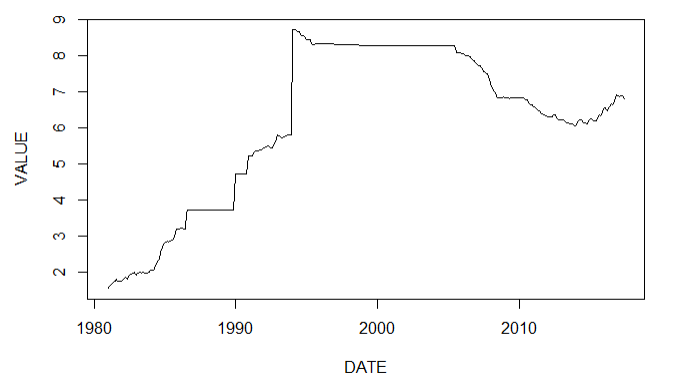
\includegraphics[width=0.6\textwidth]{monthly.png} 
\end{center}
\end{figure}

We collected the daily USD/CNY exchange rate as our data set. The data we found are already wipe out the seasonal effect so we use them directly in examining the model and further doing forecast. We divided the data into two parts one until July 21st,2016 for examine the model and the data after that date until June 9th,2017 for checking the evaluation of the models. The trend figure is shown in figure \ref{daily}.\\
\begin{figure}
\begin{center}
\caption{CNY/ USD Exchange Rate using monthly data}\label{daily}
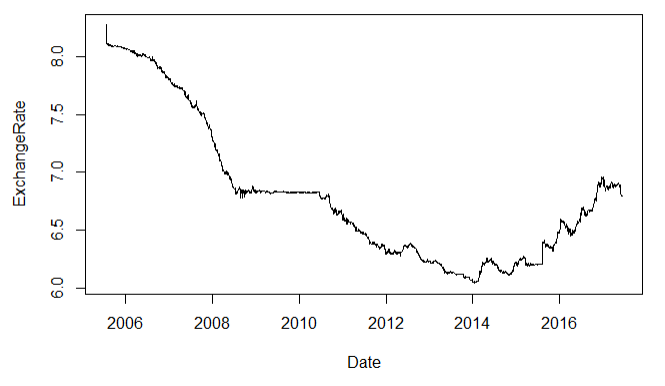
\includegraphics[width=0.6\textwidth]{daily.png} 
\end{center}
\end{figure}

\section{Model Specification}
There are usually two ways in analysing the exchange rate in time series: ARIMA model and GARCH model since they are the more general form of an ARMA model and an ARCH model. 

\subsection{ARIMA}
An ARIMA model is ARMA .\\

We first do an ADF test to check whether there exists an unit root in the serial.
\begin{lstlisting}[language=R] 
# ADF Test
origin=da$ExchangeRate
ex=origin[1:2766] # 2005-07-21 To 2016-07-21
dex=diff(ex)
m1=ar(dex,method = 'mle')
m1$order
adfTest(ex,lags=12,type=c("c"))

# Take difference
acf(dex)
pacf(dex)
\end{lstlisting}

\subsection{GARCH}

\section{Estimation and Result Analysis}

\section{Conclusions}\label{conclusions}
There is no longer \LaTeX{} example which was written by \cite{doe}.

\section{Reference}
\begin{thebibliography}{9}
\bibitem[Doe]{doe} \emph{First and last \LaTeX{} example.},
John Doe 50 B.C. 
\end{thebibliography}

\section{Appendix}
\subsection{Additional R code}
\begin{lstlisting}[language=R] 
library(readxl)
library(timeDate)
library(timeSeries)
library(TSA)
library(fUnitRoots)
library(forecast)

data <- read_excel("D:/Junior/GitHub/FDA_project_LYF/Data/MonthlyData.xls")

head(data)
dim(data)

plot(data,type="l")
\end{lstlisting}
\end{document}
